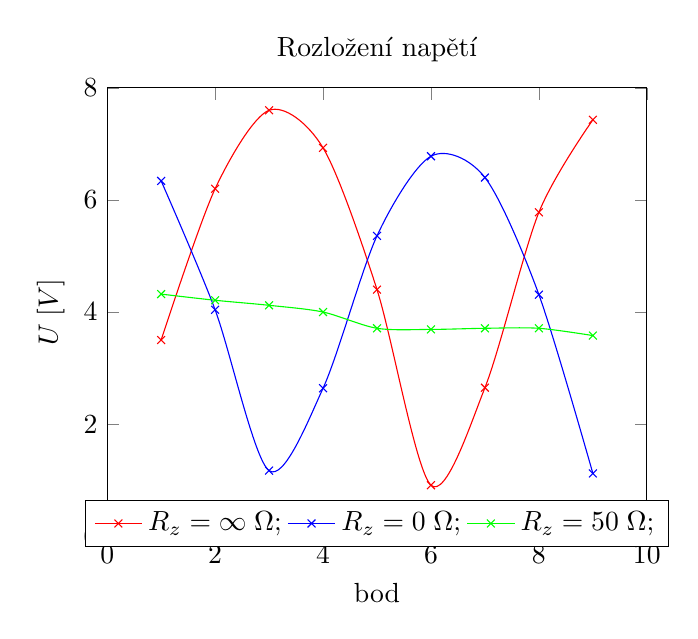
\begin{tikzpicture}
    \begin{axis}[
        title={Rozložení napětí},
        ylabel={\(U\;[V]\)},
        xlabel={bod},
        xmin=0, xmax=10,
        ymin=0, ymax=8,
        legend style={
            % area legend,
            at={(0.5,0.08)},
            anchor=north,
            legend columns=-1}]
    ]
    \addplot[
        smooth,
        color=red,
        mark=x,
        ]
        coordinates {
            (1, 3.50)
            (2, 6.20)
            (3, 7.60)
            (4, 6.93)
            (5, 4.40)
            (6, 0.91)
            (7, 2.65)
            (8, 5.78)
            (9, 7.43)
            };
    \addlegendentry{\(R_z=\infty\;\Omega\);}
    \addplot[
        smooth,
        color=blue,
        mark=x,
        ]
        coordinates {
            (1, 6.34)
            (2, 4.04)
            (3, 1.17)
            (4, 2.64)
            (5, 5.36)
            (6, 6.78)
            (7, 6.40)
            (8, 4.31)
            (9, 1.12)
        };
    \addlegendentry{\(R_z=0\;\Omega\);}
    \addplot[
        smooth,
        color=green,
        mark=x,
        ]
        coordinates {
            (1, 4.32)
            (2, 4.21)
            (3, 4.12)
            (4, 4.00)
            (5, 3.71)
            (6, 3.69)
            (7, 3.71)
            (8, 3.71)
            (9, 3.58)
        };
    \addlegendentry{\(R_z=50\;\Omega\);}
    \end{axis}
\end{tikzpicture}